\documentclass{article}

\usepackage{arxiv}

\usepackage[utf8]{inputenc} % allow utf-8 input
\usepackage[T1]{fontenc}    % use 8-bit T1 fonts
%\usepackage{hyperref}       % hyperlinks
\usepackage{url}            % simple URL typesetting
\usepackage{booktabs}       % professional-quality tables
\usepackage{amsfonts}       % blackboard math symbols
\usepackage{amsmath}
\usepackage{amssymb}
\usepackage{nicefrac}       % compact symbols for 1/2, etc.
\usepackage{microtype}      % microtypography
\usepackage{minted}

\usepackage{graphicx}
\usepackage{subcaption}

% ENVIRONMENTS
\usepackage{amsthm}
\theoremstyle{plain}
\newtheorem{definition}{Definition}[section]
\newtheorem{lemma}[definition]{Lemma}
\newtheorem{proposition}[definition]{Proposition}
\newtheorem{corollary}[definition]{Corollary}
\theoremstyle{remark}
\newtheorem{remark}[definition]{Remark}
\newtheorem{example}[definition]{Example}

% TEXT-MODE MACROS
\newcommand{\IN}{\mathbb{N}}
\newcommand{\IR}{\mathbb{R}}
\newcommand{\IZ}{\mathbb{Z}}
\newcommand{\union}{\cup}
\newcommand{\Union}{\bigcup}
\newcommand{\code}{\texttt} % for use as \code{test()}
\newcommand{\defn}{\emph} % for use as \defn{...}

% MATH-MODE MACROS
\newcommand{\qtext}[1]{\quad\text{#1}\quad} % for use as \def{...} inside text
\newcommand{\lra}{\longrightarrow}
\newcommand{\floor}[1]{\lfloor#1\rfloor}
\newcommand{\abs}[1]{|#1|}
\newcommand{\eps}{\epsilon}


\title{circllhist}

\subtitle{The Circonus Log-Linear Histogram}

\author{
  Heinrich Hartmann \\
  \texttt{heinrich.hartmann@circonus.com} \\
  Circonus \\
  \And
  Theo Schlossnagle \\
  \texttt{theo.schlossnagle@circonus.com} \\
  Circonus
}


\begin{document}

\maketitle

\begin{abstract}
  The circllhist histogram is a simple, fast and memory efficient data structure for capturing
  and processing large number of samples, that is particularly suited for applications in
  IT infrastructure monitoring.

  The circllhist allows arbitrary merging of pre-aggregated data without additional loss of accuracy,
  and the approximation of percentiles with low expected error and a-priori bounded maximal error.

  Open-source implementations are available for C/lua/python/Go/Java/JavaScript.
\end{abstract}

\tableofcontents

\section{Introduction}
The circllhist is a histogram data structure that allows the representation of an virtually
unlimited amount of data with bounded memory consumption, and precise a-priori bounds for the
accuracy of derived statistics.

In this note we will describe the data structure ...

\section{Related Work}

\subsection{HDR Histograms}

\subsection{t-digest}

\subsection{DD-sketches}

\section{Abstract Histograms}

\subsection{Binnings}

\begin{definition}
  An binning $B$ is a set of disjoint intervals (``bins'') $B[i], i\in I$, indexed by a
  finite or countably infinite set $I$.
  The union of all bins in a binning is called the domain, $Dom(B)$.
  \begin{align*}
    \Union_{i \in I} B[i] = Dom(B) \subset \IR,\quad B[i] \cap B[j] = \emptyset \qtext{for} i \neq j \in I.
  \end{align*}
  The map, that associates to $x \in Dom(B)$ the index $i$ of the unique bin with $x \in B[i]$,
  is called \defn{binning map}
  and denoted as follows:
  \begin{align*}
    bin: Dom(B) \lra I, x \mapsto bin(x) \qtext{with} x \in B[bin(x)]
  \end{align*}
\end{definition}

\begin{example}
  The linear binning of $\IR$ is given by $I = \IZ$, $B_i = [i, i+1)$, with $bin(x)=\floor{x}$.
\end{example}

\begin{example}
  The log-linear binning with basis $b$ of $\IR_{>0}$ is given by $I=\IZ$, $B_i = [b^i, b^{i+1})$, with $bin(x)=\floor{\log_b(x)}$.
\end{example}

\begin{remark}
  The binning map $Dom(B) \lra I$ uniquely determines the binning $B$, via
  \begin{align*}
    B[i] = bin^{-1}\{ i \} = \{ x \in Dom(B) \,|\, bin(x) = i \}.
  \end{align*}
  Given a map $f:\IR \supset D \lra I$, there is a unique binning with binning map $f$, if the fibers $f^{-1}\{i\}, i \in I$ are intervals.
\end{remark}

\subsection{Log-Linear Binnings}
\newcommand{\float}{\mathrm{float}}
\newcommand{\bin}{\mathrm{bin}}

Let $b,p \in \IN$ be integers with $b\geq 2, p \geq 1$.
The \defn{base-$b$ precision-$p$ log-linear binning} has a bin boundary at each base-$b$ floating point number with $p$ significant digits.
We will be mainly interested in the decimal precision-2 binning, which has it's bin boundaries at the base-10 floating point numbers with two significant digits.

Recall that floating point numbers are represented by sign, mantissa and exponent.
For example the number
\begin{align*}
  \underbrace{+}_{\text{sign}} \underbrace{6.6}_{\text{mantissa}} \cdot {\underbrace{10}_{\text{base}}\hspace{.5em}}^{-36} \hspace{-2em}\underbrace{\hspace{.5em}}_{\text{exponent}}.
\end{align*}
has sign $s=+1$, mantissa $d=66$ and exponent $e=-36$.

\begin{definition}
  For each tuple $(s,d,e)$ of integers with $s=\pm1$ we associate a real number:
  \begin{align*}
    \float_{b,p}(s,d,e) := s \cdot \frac{d}{b^{p-1}} \cdot b^e = s \cdot d \cdot b^{e-p+1}
  \end{align*}
  By convention we set $\float_{b,p}(0,0,0)=0$.
\end{definition}

\begin{example}
  We have
  \begin{align*}
    \float_{10,2}(+1,66,-36) = 66/10 \cdot 10^{-36}  = 6.6 \cdot 10^{-36}.
  \end{align*}
  The number $0$ is represented as $\float_{b,p}(0,0,0) = 0$.
  The number $1$ is represented as $\float_{b,p}(+1,b^{p-1},0) = 1$.
\end{example}

\begin{definition} \label{hdrdef}
  The base-$b$ precision-$p$ log-linear binning has index set
  \begin{align*}
    I_{b,p} = \{\, (s,d,e) \,|\, s,d,e \in \IZ \,\text{with}\, s=d=e=0 \,\text{or}\, s=\pm1, b^{p-1} \leq d < b^p \,\}
  \end{align*}
  and bins $B[s,d,e]$ defined by
  \begin{align*}
    B[+1,d,e] &= \mathopen[\,\float_{b,p}(+1,d,e), \float_{b,p}(+1,d+1,e)\,\mathopen), \\
    B[0,0,0]  &= \{ 0 \}, \\
    B[-1,d,e] &= \mathopen(\,\float_{b,p}(-1,d+1,e), \float_{b,p}(-1,d+1,e)\,\mathopen].
  \end{align*}
\end{definition}

\begin{remark} For the largest allowable $d=b^{p}-1$ we have $(s,d+1,e) \neq I_{b,p}$, but
  \begin{align*}
    \float_{b,p}(s,d + 1,e) = \float_{b,p}(s, b^p ,e) = \float_{b,p}(s, b^{p-1}, e+1)
  \end{align*}
  with $(s, b^{p-1}, e) \in I_{b,p}$.
  So the bin boundaries can always be chosen from the index set $I_{b,p}$.
\end{remark}

It's not clear from the above definition that the bins are disjoint and cover the real axes.
The rest of this section is devoted to demonstrating this and determining the binning map.

\begin{definition}
  For $x\in\IR, x\neq 0$, we define the following functions:
  \begin{align*}
    s(x) := sign(x), \quad
    e(x) := \floor{\log_b\abs{x}}, \quad
    d(x) := \floor{\abs{x} \cdot b^{-e(x)+p-1}} \quad
    \delta(x) := \abs{x} \cdot b^{-e(x)+p-1} - d(x).
  \end{align*}
  Moreover we set $s(0) = e(0) = d(0) = \delta(0) = 0$.
\end{definition}

\begin{lemma} \label{floatlem}
  (A) For $x \neq 0$ we have
  \begin{align*}
    b^{p-1} \leq d(x) < b^p \qtext{and} 0 \leq \delta(x) < 1.
  \end{align*}

  (B) For $x \in \IR$ we have
  \begin{align*}
    x = s(x) \cdot (d(x) + \delta(x)) \cdot b^{e(x) - p + 1}
  \end{align*}

  (C) If $x \neq 0$ is represented as
  \begin{align*}
    x = s \cdot (d + \delta) \cdot b^{e - p + 1}
  \end{align*}
  with $s \in \{\pm 1\}$, $\delta \in [0,1)$ and $d \in \IZ$ with $b^{p-1} \leq d < b^p$, then
  \begin{align*}
    s = s(x), \quad d = d(x), \quad e = e(x) \qtext{and} \delta = \delta(x).
  \end{align*}
\end{lemma}

\begin{proof}
  We start with claim (B). For $x=0$ we have $s(0) = 0$ hence the equation holds.
  For $x \neq 0$, we have
  \begin{align*}
    x = sign(x) |x| = sign(x) \abs{x} \cdot b^{-e(x)+p-1} \cdot b^{e(x)-p+1} = s(x) \cdot (d(x) + \delta(x)) \cdot b^{e(x)-p+1}
  \end{align*}
  as claimed.

  Ad A) Note that $\delta(x)$ is of the form $y - \floor{y}$ and hence in $[0,1)$.

  For $x \neq 0$, we write $|x| = b^{log_b|x|} = b^{e(x) + \eps}$, with $\eps \in [0,1)$.
  Hence $\abs{x} / b^{e(x)} = b^\eps \in [1,b)$ and
  \begin{align*}
     d(x) + \delta(x) = \abs{x} \cdot b^{-e(x)+p-1} = \abs{x} / b^{e(x)} \cdot b^{p-1} \in [b^{p-1},b^p).
  \end{align*}
  It follows that also $d(x) = \floor{d(x) + \delta(x)} \in [ b^{p-1}, b^p )$
  since both $b^{p-1}$ and $b^p$ are integers.

  Ad C) We have
  \begin{align*}
    s(x) &= sign(s \cdot (d + \delta) \cdot b^{e-p+1}) = s, \\
    e(x) &= \floor{ \log_b \abs{s \cdot (d + \delta) \cdot b^{e-p+1}} } = \floor{\log_b((d+\delta)/b^{p-1})} + e = e, \\
    d(x) &= \floor{\abs{ s \cdot (d + \delta) \cdot b^{e-p+1} } \cdot b^{p-1-e(x)}} = \floor{d + \delta} = d, \\
    \delta(x) &= (d + \delta) - \floor{d + \delta} = \delta.
  \end{align*}
  In the second equation we used, that $b^{p-1} \leq d < b^p$ and this inequality between integers
  not changed by adding a small real number $\delta \in [0,1)$ to $d$.
  Hence $1 \leq (d+\delta) /  b^{p-1} < b$ and $0 \leq log_b((d+\delta) /  b^{p-1}) < 1$.
\end{proof}

\begin{corollary}
  A number $x \in \IR$ is of the form
  \begin{align*}
    x = \float_{b,p}(s,d,e)
  \end{align*}
  for some integers $s,d,e$ with $b^{p-1} \leq d < b^p$, $s \in \{\pm 1\}$, if and only if $\delta(x) = 0$.
  In this case
  \begin{align*}
    s = s(x), \quad d = d(x), \quad e = e(x).
  \end{align*}
\end{corollary}
\begin{proof}
  By the Lemma \ref{floatlem} (B), we have
  \begin{align*}
    x = s(x) (d(x) + \delta(x)) b^{e(x)-p+1} = \float_{b,p}(s(x), d(x), e(x)) + \delta(x) \cdot b^{e(x) - p + 1},
  \end{align*}
  so $\delta(x) = 0$ implies $x = \float_{b,p}(s(x),d(x),e(x))$.

  Conversely, if $x = \float_{b,p}(s,d,e)$ then $s = s(x), d = d(x), e = e(x), \delta(x) = 0$ by \ref{floatlem} (C).
\end{proof}

\begin{proposition} \label{hdrprop}
  For $x \in \IR, (s,d,e) \in I_{b,p}$ we have $x \in B[s,d,e]$ if and only if $\bin_{b,p}(x) = (s,d,e)$.
\end{proposition}
\begin{proof}
  Assume that $x \in B[+1,d,e]$. By definition of $B[1,d,e]$ we have
  \begin{align*}
    \float_{b,p}(+1,d,e) = & d \cdot b^{e-p+1} \leq x < \float_{b,p}(+1,d+1, e) = (d+1) \cdot b^{e-p+1}.
  \end{align*}
  Dividing by $b^{e-p+1}$ we find that $\delta := x/b^{e-p+1} - d$ lies in $[0,1)$.
  Solving for $x$ we find $x = (d + \delta) \cdot b^{e-p+1}$, and it follows by
  Lemma \ref{floatlem} (C), that $d=d(x), e=e(x), \delta = \delta(x)$, so $\bin_{b,p}(x) = (1,d,e)$.

  Conversely if $\bin_{b,p}(x) = (1,d,e)$, then $x = (d + \delta(x)) \cdot b^{e - p + 1}$
  \begin{align*}
      \float_{b,p}(1,d,e) = (d + 0) \cdot b^{e - p + 1} \leq (d + \delta(x)) \cdot b^{e - p + 1} <  (d + 1) \cdot b^{e - p + 1} = \float_{b,p}(1,d+1,e)
  \end{align*}
  and hence $x \in B[1,d,e]$.

  For $x = 0$ we have $bin(x) = (0,0,0)$ by definition.
  Conversely if $bin(x) = (0,0,0)$ then $s(x) = 0$ so $x = 0$.

  The case $x < 0$ can be derived from the first equation using the identities $bin(-x)=(-s(x),d(x),e(x))$ and $B[-1,d,e] = -B[1,d,e]$.
\end{proof}

\begin{corollary}
  (A) The log-linear bins $B[s,d,e]$ are precisely the fibers of the map
  \begin{align*}
    bin_{b,p}: \IR \lra I_{b,p}, \quad x \mapsto bin_{b,p}(x) = (s(x), d(x), e(x) ),
  \end{align*}
  i.e. $\bin_{b,p}^{-1}\{(s,d,e)\} = B[s,d,e].$

  (B) The bins $B[s,d,e], (s,d,e) \in I_{b,p}$ are disjoint and collectively cover the real axes $\IR$.

  (C) log-linear histograms are well defined by Definition \ref{hdrdef} and have bin mapping $\bin_{b,p}: \IR \lra I_{b,p}$.

  (D) The bin sizes for the log-linear binning is given by $size(B[s,d,e]) = b^{e-p+1}$.
\end{corollary}

\begin{proof}
  (A) is a reformulation of Proposition \ref{hdrprop}.
  (B) follows from (A) since the fibers $f^{-1}\{x\}$ of any map $f:X \rightarrow Y$ are disjoint and cover the domain $X$.
  (C) follows from (B) and (A).

  (D) follows directly from the definition since $\float_{b,p}(1,d+1,e)-\float_{b,p}(1,d,e) = b^{e-p+1}$.
\end{proof}

\subsection{Histogram Summaries}
Given a binning $B_i, i\in I$ of $D \subset \IR$, and  dataset $X=(x_1,\dots, x_N) $ with values in
$D \subset \IR$, we associate a count function:

\begin{align*} c_D(i) = \# \{ j | y_j \in B_i \} \end{align*}

The datum of a binning $B_i,i\in I$ and a count function $c_i,\in I$, is called a histogram summary of $X$.

\subsection{Imlementation}

\begin{itemize}
\item HdrHistogram
\item t-digest
\end{itemize}

\section{The Circllhist Datastructure}
\begin{minted}[frame=lines,framesep=2mm]{c}

struct histogram {
  uint16_t allocd;
  uint16_t used;
  struct hist_bv_pair *bvs;
};

struct hist_bv_pair {
  hist_bucket_t bucket;
  uint64_t count;
};

typedef struct hist_bucket {
  int8_t val;
  int8_t exp;
} hist_bucket_t;
\end{minted}

\section{Histogram Operations}

\subsection{Merging}

\subsection{Mean Values}

\subsection{Percentiles}

\section{Evaluation}

\subsection{Datasets}

\begin{figure}
    \begin{subfigure}[b]{0.9\textwidth}
        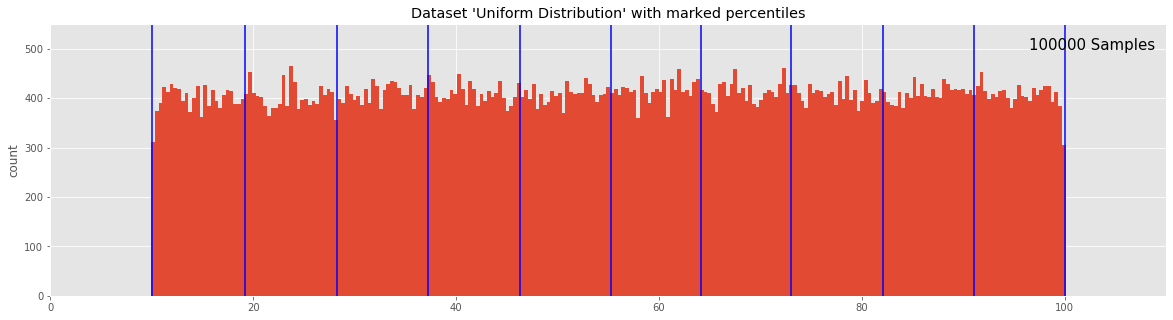
\includegraphics[width=\textwidth]{evaluation/images/Uniform_Distribution_distribution_percentiles.png}
        \caption{Uniform Distribution}
    \end{subfigure}
    \begin{subfigure}[b]{0.9\textwidth}
        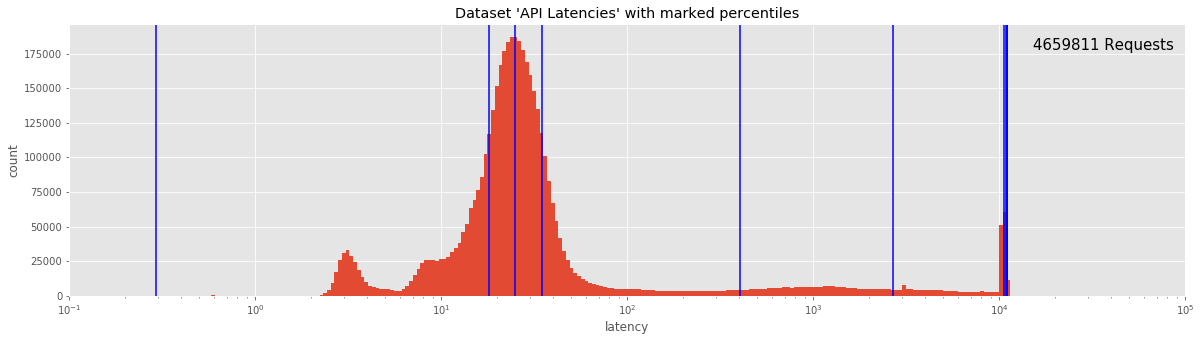
\includegraphics[width=\textwidth]{evaluation/images/API_Latencies_distribution_percentiles.png}
        \caption{API Latencies}
    \end{subfigure}
    \begin{subfigure}[b]{0.9\textwidth}
        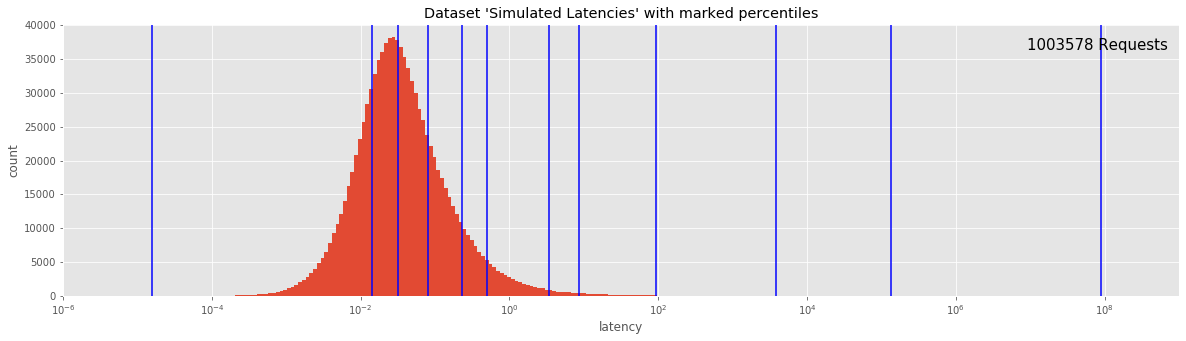
\includegraphics[width=\textwidth]{evaluation/images/Simulated_Latencies_distribution_percentiles.png}
        \caption{Simulated API Latencies}
    \end{subfigure}
    \caption{Datasets}
\end{figure}

\subsection{Size}


Two Points\\

\begin{tabular}{lrrrrrrr}
\toprule
{} &  exact &  tdigest &   hdr &   dd &  circllhist/type-1 &  circllhist/type-7 &  prom1 \\
\midrule
bsize &    171 &       64 &  30.0 &  605 &               12.0 &               12.0 &    235 \\
\bottomrule
\end{tabular}


Uniform\\

\begin{tabular}{lrrrrrr}
\toprule
{} &   exact &  prom &    hdr &  tdigest &   dd &  circllhist \\
\midrule
Uniform Distribution &  800000 &    96 &  621.0 &     2224 &  716 &       453.0 \\
\bottomrule
\end{tabular}


API Latencies\\

\begin{tabular}{lrrrrrr}
\toprule
{} &     exact &  prom &     hdr &  tdigest &    dd &  circllhist \\
\midrule
API Latencies &  37278488 &    96 &  2994.0 &     2368 &  1902 &      1866.0 \\
\bottomrule
\end{tabular}


Simulated API Latency Data\\

\begin{tabular}{lrrrrrr}
\toprule
{} &    exact &  prom &      hdr &  tdigest &    dd &  circllhist \\
\midrule
Simulated Latencies &  8028624 &    96 &  16455.0 &     2096 &  3428 &      3396.0 \\
\bottomrule
\end{tabular}


\subsection{Performance}

\begin{figure}
    \centering
    \begin{subfigure}[b]{0.3\textwidth}
        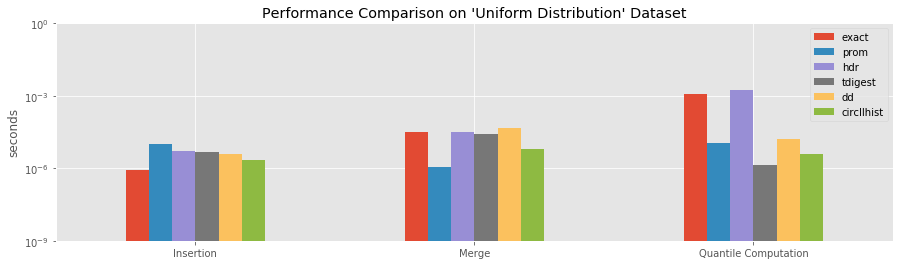
\includegraphics[width=\textwidth]{evaluation/images/Uniform_Distribution_perf.png}
        \caption{Uniform Distribution}
    \end{subfigure}
    ~
    \begin{subfigure}[b]{0.3\textwidth}
        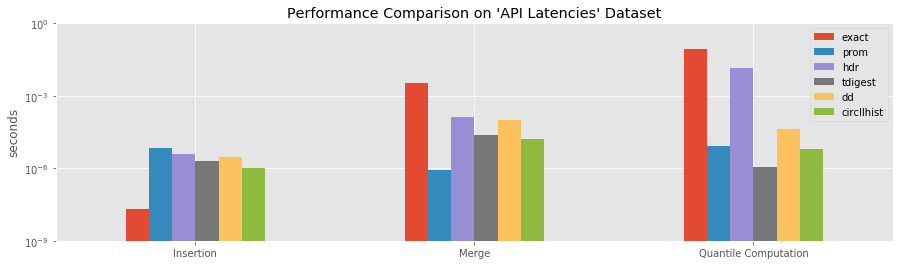
\includegraphics[width=\textwidth]{evaluation/images/API_Latencies_perf.png}
        \caption{API Latencies}
    \end{subfigure}
    ~
    \begin{subfigure}[b]{0.3\textwidth}
        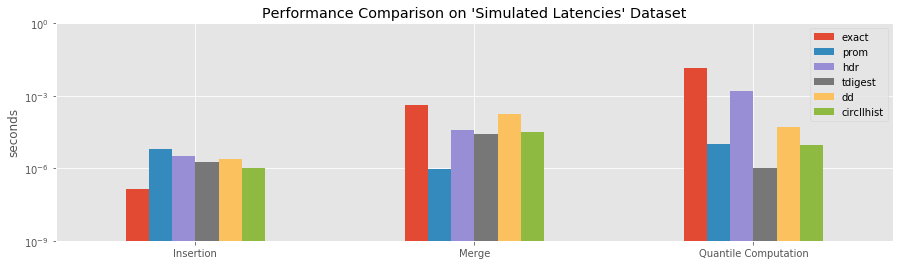
\includegraphics[width=\textwidth]{evaluation/images/Simulated_Latencies_perf.png}
        \caption{Simulated API Latencies}
    \end{subfigure}
    \caption{Performance Comparison}
\end{figure}


Two Points\\

\begin{tabular}{lrrrrrrr}
\toprule
{} &     exact &      prom &   tdigest &       hdr &        dd &  circllhist/type-1 &  circllhist/type-7 \\
\midrule
insert    &  0.000216 &  0.000807 &  0.018123 &  0.000449 &  0.000102 &           0.000825 &           0.000384 \\
merge     &  0.000003 &  0.000087 &  0.000027 &  0.000192 &  0.000008 &           0.000004 &           0.000004 \\
quantiles &  0.000088 &  0.000241 &  0.000024 &  0.239204 &  0.000256 &           0.000059 &           0.000060 \\
\bottomrule
\end{tabular}


Uniform\\

\begin{tabular}{lrrrrrr}
\toprule
{} &  exact &  prom &    hdr &  tdigest &   dd &  circllhist \\
\midrule
Insertion            &    0.9 &  10.5 &    7.7 &      4.6 &  3.8 &         2.2 \\
Merge                &   33.1 &   1.1 &  129.0 &     26.9 & 45.8 &         6.3 \\
Quantile Computation & 1180.3 &  11.3 & 9684.9 &      1.4 & 17.1 &         3.8 \\
\bottomrule
\end{tabular}


API Latencies\\

\begin{tabular}{lrrrrrr}
\toprule
{} &   exact &  prom &    hdr &  tdigest &    dd &  circllhist \\
\midrule
Insertion            &     0.0 &   6.9 &    3.7 &      2.0 &   3.0 &         1.0 \\
Merge                &  3487.6 &   0.9 &   34.1 &     24.0 & 104.6 &        16.1 \\
Quantile Computation & 83773.2 &   8.3 & 1931.4 &      1.1 &  42.6 &         6.1 \\
\bottomrule
\end{tabular}


Simulated API Latency Data\\

\begin{tabular}{lrrrrrr}
\toprule
{} &   exact &  prom &     hdr &  tdigest &    dd &  circllhist \\
\midrule
Insertion            &     0.1 &   6.5 &     3.5 &      1.9 &   2.5 &         1.0 \\
Merge                &   415.4 &   1.0 &   135.6 &     27.1 & 185.7 &        31.7 \\
Quantile Computation & 14222.5 &  10.0 & 11198.1 &      1.1 &  51.4 &         8.9 \\
\bottomrule
\end{tabular}


\subsection{Accuracy}

\begin{figure}
  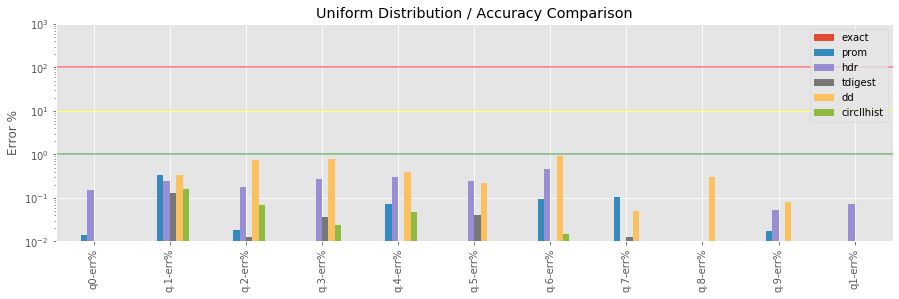
\includegraphics[width=\textwidth]{evaluation/images/Uniform_Distribution_accuracy.png}
  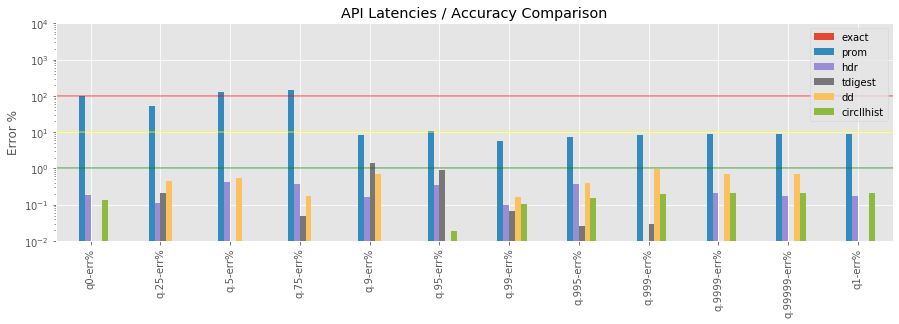
\includegraphics[width=\textwidth]{evaluation/images/API_Latencies_accuracy.png}
  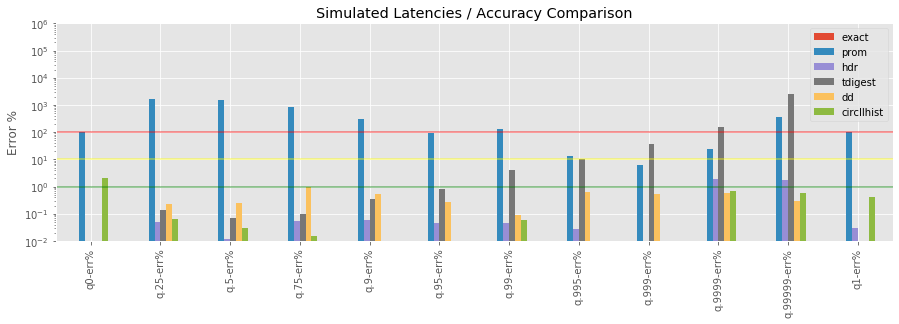
\includegraphics[width=\textwidth]{evaluation/images/Simulated_Latencies_accuracy.png}
  \caption{Accuracy Comparison}
\end{figure}


Two Points\\

\begin{tabular}{lrrrrrrr}
\toprule
{} &  exact &    prom &  tdigest &         hdr &        dd &  circllhist/type-1 &  circllhist/type-7 \\
\midrule
q0-err\%   &    0.0 &    1.00 &      0.0 &    0.007793 &  0.000000 &                5.0 &                5.0 \\
q.05-err\% &    0.0 &    0.85 &      0.0 &    0.059316 &  0.746967 &                5.0 &                5.0 \\
q.1-err\%  &    0.0 &    0.70 &      0.0 &    0.059316 &  0.746967 &                5.0 &                5.0 \\
q.15-err\% &    0.0 &    0.55 &      0.0 &    0.059316 &  0.746967 &                5.0 &                5.0 \\
q.2-err\%  &    0.0 &    0.40 &      0.0 &    0.059316 &  0.746967 &                5.0 &                5.0 \\
q.25-err\% &    0.0 &    0.25 &      0.0 &    0.059316 &  0.746967 &                5.0 &                5.0 \\
q.3-err\%  &    0.0 &    0.10 &     90.0 &    0.059316 &  0.746967 &                5.0 &                5.0 \\
q.35-err\% &    0.0 &    0.05 &    180.0 &    0.059316 &  0.746967 &                5.0 &                5.0 \\
q.4-err\%  &    0.0 &    0.20 &    270.0 &    0.059316 &  0.746967 &                5.0 &                5.0 \\
q.45-err\% &    0.0 &    0.35 &    360.0 &    0.059316 &  0.746967 &                5.0 &                5.0 \\
q.5-err\%  &    0.0 &    0.50 &    450.0 &    0.059316 &  0.746967 &                5.0 &                5.0 \\
q.55-err\% &    0.0 &  899.15 &    540.0 &    0.059316 &  0.746967 &              950.0 &                5.0 \\
q.6-err\%  &    0.0 &  899.30 &    630.0 &    0.059316 &  0.746967 &              950.0 &                5.0 \\
q.65-err\% &    0.0 &  899.45 &    720.0 &    0.059316 &  0.746967 &              950.0 &                5.0 \\
q.7-err\%  &    0.0 &  899.60 &    810.0 &    0.059316 &  0.746967 &              950.0 &                5.0 \\
q.75-err\% &    0.0 &  899.75 &    900.0 &  900.190509 &  0.746967 &              950.0 &                5.0 \\
q.8-err\%  &    0.0 &  899.90 &    900.0 &  900.190509 &  0.746967 &              950.0 &                5.0 \\
q.85-err\% &    0.0 &  900.05 &    900.0 &  900.190509 &  0.746967 &              950.0 &                5.0 \\
q.9-err\%  &    0.0 &  900.20 &    900.0 &  900.190509 &  0.746967 &              950.0 &                5.0 \\
q.95-err\% &    0.0 &  900.35 &    900.0 &  900.190509 &  0.746967 &              950.0 &                5.0 \\
q1-err\%   &    0.0 &    0.05 &      0.0 &    0.019051 &  0.000000 &                5.0 &                5.0 \\
\bottomrule
\end{tabular}


Uniform\\

\begin{tabular}{lrrrrr}
\toprule
{} &  prom &   hdr &  tdigest &    dd &  circllhist \\
\midrule
q0-err\%  & 0.014 & 0.156 &    0.000 & 0.000 &       0.005 \\
q.1-err\% & 0.339 & 0.248 &    0.129 & 0.342 &       0.160 \\
q.2-err\% & 0.018 & 0.178 &    0.013 & 0.736 &       0.069 \\
q.3-err\% & 0.006 & 0.273 &    0.036 & 0.794 &       0.024 \\
q.4-err\% & 0.074 & 0.297 &    0.003 & 0.394 &       0.048 \\
q.5-err\% & 0.000 & 0.243 &    0.040 & 0.216 &       0.007 \\
q.6-err\% & 0.094 & 0.468 &    0.006 & 0.931 &       0.015 \\
q.7-err\% & 0.105 & 0.006 &    0.013 & 0.050 &       0.000 \\
q.8-err\% & 0.004 & 0.010 &    0.001 & 0.307 &       0.009 \\
q.9-err\% & 0.017 & 0.053 &    0.006 & 0.081 &       0.000 \\
q1-err\%  & 0.000 & 0.073 &    0.000 & 0.000 &       0.001 \\
\bottomrule
\end{tabular}


API Latencies\\

\begin{tabular}{lrrrrr}
\toprule
{} &    prom &   hdr &  tdigest &    dd &  circllhist \\
\midrule
q0-err\%      & 100.000 & 0.038 &    0.000 & 0.000 &       0.134 \\
q.25-err\%    &  52.671 & 0.035 &    0.216 & 0.460 &       0.000 \\
q.5-err\%     & 126.469 & 0.038 &    0.000 & 0.538 &       0.003 \\
q.75-err\%    & 145.163 & 0.061 &    0.049 & 0.171 &       0.001 \\
q.9-err\%     &   8.230 & 0.007 &    1.382 & 0.685 &       0.006 \\
q.95-err\%    &  10.636 & 0.023 &    0.907 & 0.006 &       0.019 \\
q.99-err\%    &   5.662 & 0.031 &    0.066 & 0.164 &       0.105 \\
q.995-err\%   &   7.313 & 0.064 &    0.026 & 0.399 &       0.155 \\
q.999-err\%   &   8.584 & 0.010 &    0.030 & 0.979 &       0.202 \\
q.9999-err\%  &   8.862 & 0.019 &    0.007 & 0.715 &       0.216 \\
q.99999-err\% &   8.891 & 0.050 &    0.003 & 0.683 &       0.216 \\
q1-err\%      &   8.894 & 0.047 &    0.000 & 0.000 &       0.217 \\
\bottomrule
\end{tabular}


Simulated API Latency Data\\

\begin{tabular}{lrrrrr}
\toprule
{} &     prom &   hdr &  tdigest &    dd &  circllhist \\
\midrule
q0-err\%      &  100.000 & 0.407 &    0.000 & 0.000 &       2.110 \\
q.25-err\%    & 1706.372 & 0.232 &    0.141 & 0.238 &       0.062 \\
q.5-err\%     & 1523.356 & 0.012 &    0.069 & 0.243 &       0.029 \\
q.75-err\%    &  857.929 & 0.054 &    0.101 & 0.957 &       0.016 \\
q.9-err\%     &  296.620 & 0.689 &    0.342 & 0.546 &       0.009 \\
q.95-err\%    &   95.263 & 0.632 &    0.813 & 0.277 &       0.004 \\
q.99-err\%    &  133.561 & 0.146 &    4.152 & 0.087 &       0.059 \\
q.995-err\%   &   13.454 & 0.029 &   10.259 & 0.649 &       0.008 \\
q.999-err\%   &    6.136 & 0.406 &   36.221 & 0.519 &       0.002 \\
q.9999-err\%  &   23.154 & 1.933 &  149.000 & 0.599 &       0.670 \\
q.99999-err\% &  355.293 & 2.224 & 2559.294 & 0.301 &       0.570 \\
q1-err\%      &   98.875 & 0.347 &    0.000 & 0.000 &       0.409 \\
\bottomrule
\end{tabular}



\bibliographystyle{unsrt}
\begin{thebibliography}{1}

\bibitem{t-digest}
George Kour and Raid Saabne.
\newblock Real-time segmentation of on-line handwritten arabic script.
\newblock In {\em Frontiers in Handwriting Recognition (ICFHR), 2014 14th
  International Conference on}, pages 417--422. IEEE, 2014.

\bibitem{HdrHistogram}
George Kour and Raid Saabne.
\newblock Real-time segmentation of on-line handwritten arabic script.
\newblock In {\em Frontiers in Handwriting Recognition (ICFHR), 2014 14th
  International Conference on}, pages 417--422. IEEE, 2014.

\bibitem{kour2014real}
George Kour and Raid Saabne.
\newblock Real-time segmentation of on-line handwritten arabic script.
\newblock In {\em Frontiers in Handwriting Recognition (ICFHR), 2014 14th
  International Conference on}, pages 417--422. IEEE, 2014.

\end{thebibliography}
\end{document}
